\documentclass[11pt]{article}
\usepackage[utf8]{inputenc}
\usepackage[french]{babel}
\usepackage{graphicx}
\usepackage[T1]{fontenc}
%\usepackage{amss}
\usepackage{amsmath}
\usepackage{amsfonts}
\usepackage{amssymb}

\newcommand\comment{}
\def\N{\mathbb N}
\def\R{\mathbb R}
\def\Q{\mathbb Q}
\def\Z{\mathbb Z}
\begin{document}
\title{PARTIEL I31, Dijon, 2016}
\date{}\maketitle

{\bf Vous avez droit à VOS documents.}

{\bf Recopiez toutes les figures sur votre copie d'examen.}

\section{Problème 1~: dates au plus tôt et au plus tard}

Recopiez ce graphe sur votre feuille d'examen. Indiquez les dates au plus tôt et au plus tard sur les sommets du graphe, 
et soulignez le chemin critique. 

\begin{center}
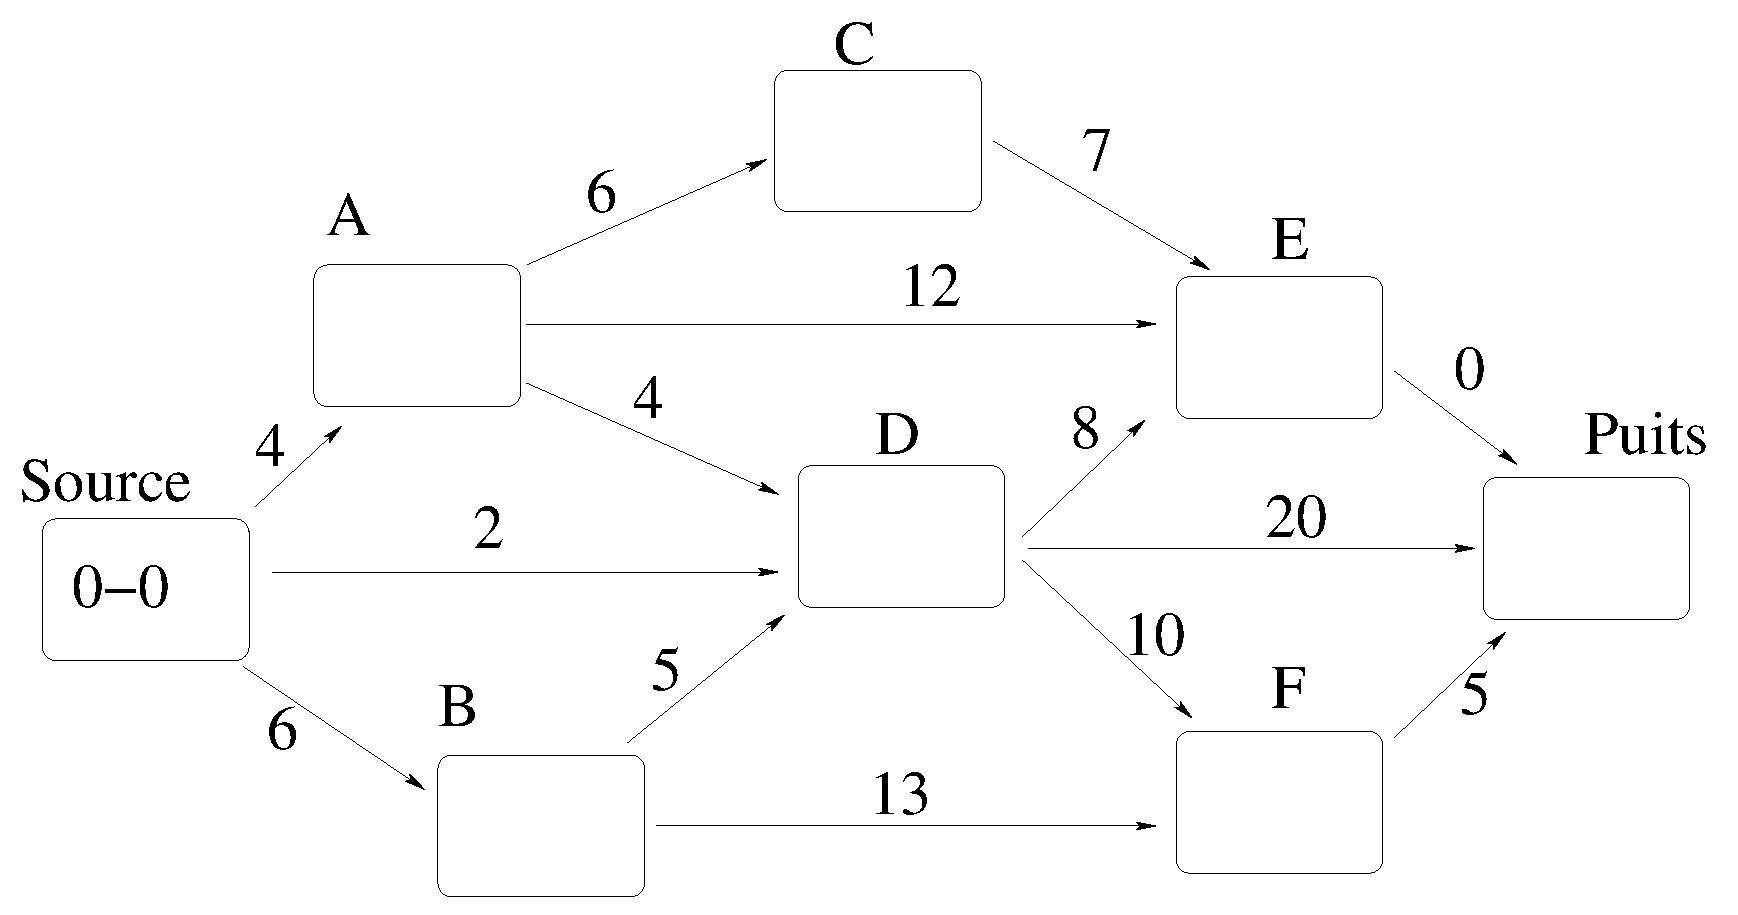
\includegraphics[width=0.7\linewidth]{critique2.eps}
\end{center}

Quel problème concernant des séquences a été réduit en cours à un problème de
dates au plus tôt et au plus tard~?

\section{Problème 2~: tri topologique}
Redessinez le graphe ci-dessous pour que tous les arcs aillent de gauche à droite (comme ceci~: $\rightarrow$).  Quels sont les premiers sommets possibles~?
Quels sont les derniers sommets possibles~? Pourquoi~?
\begin{center}
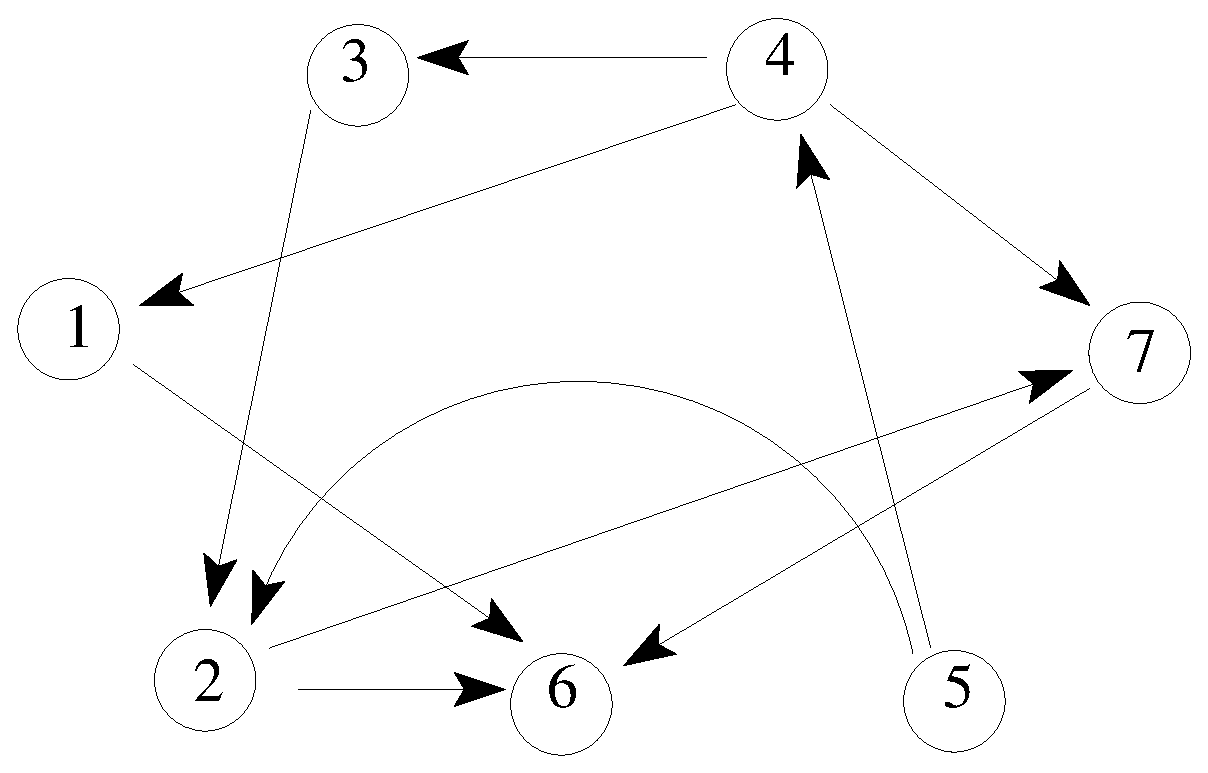
\includegraphics[width=0.6\linewidth]{tritopologique.eps}
\end{center}

\section{Problème 3~: composantes fortement connexes}
Entourez les composantes fortement connexes.
Dessinez le graphe réduit (chaque sommet du graphe réduit représente une CFC).

\begin{center}
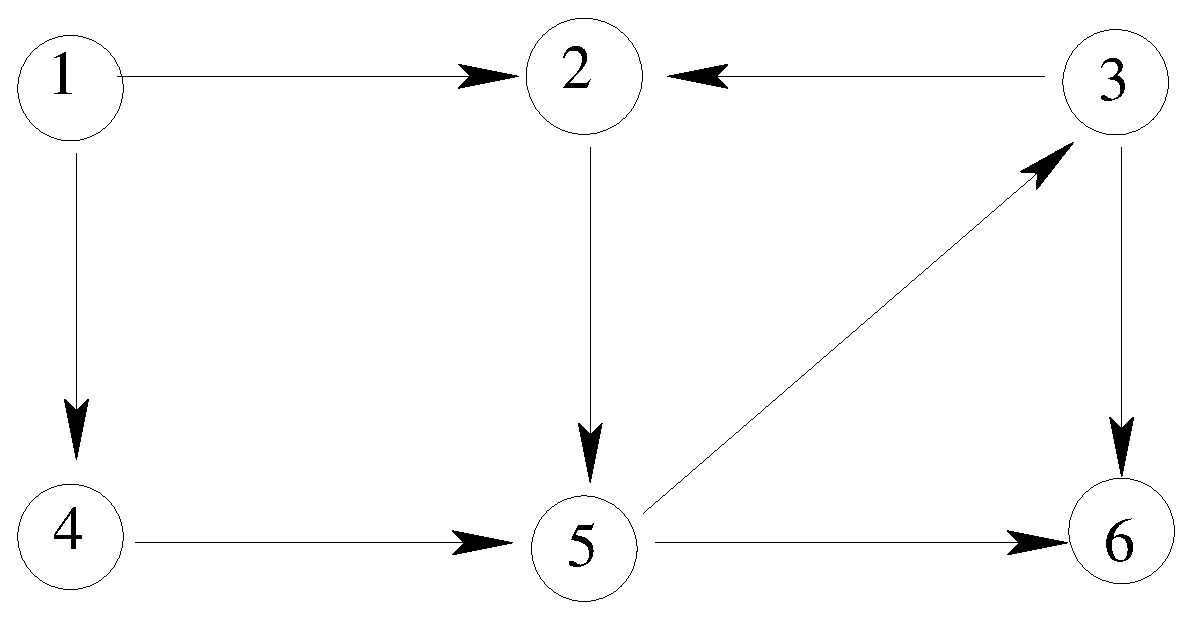
\includegraphics[width=0.55\linewidth]{cfc.eps}
\end{center}

\section{Problème 4~: Euclide et Bézout}
Calculez, avec l'algorithme d'Euclide généralisé, $(x, y, g)$, tels que $g$ soit le PGCD de 72 et 39, 
et que
$72x+39y=g$. 
Donnez le détail de vos calculs (comme en TD), par exemple dans un tableau, ou avec des produits matriciels.

Cet algorithme donne le couple $(x, y)$ tel que
$x^2+y^2$ soit minimal.  
Donnez une formule avec un paramètre $t\in\Z$  permettant de générer toutes les paires  $(x, y)$ telles
que $72x+39y=g$. 

\section{Problème 5}
Rappel~: Pour calculer efficacement la séquence de Fibonacci, définie par
$F(0)=0, F(1)=1, F(n)= F(n-1)+F(n-2)$, on considère l'expression matricielle~:

\begin{eqnarray*}
 \left( \begin{array}{c} F(n) \\
 F(n-1)
\end{array}\right) &=& 
\left( \begin{array}{cc}  1 & 1 \\
1 & 0
\end{array}\right) \left(\begin{array}{c} F(n-1) \\
 F(n-2)\end{array}\right)   \\
&=& \left( \begin{array}{cc}  1 & 1 \\
1 & 0
\end{array}\right)^{n-1} \left(\begin{array}{c} F(1)\\
F(0)\end{array}\right)
\end{eqnarray*}

Pour calculer rapidement la séquence~: $G(0)=1, G(1)=4, G(n)=2\times G(n-1)+n+1$, quelle expression matricielle faut-il considérer~? Vous pouvez compléter la matrice ci-dessous~:

$$
 \left( \begin{array}{c}
G(n) \\
n\\
1\end{array}\right) = \left( \begin{array}{ccc}
\quad & \quad & \quad \\
\quad & \quad & \quad \\
\quad & \quad & \quad \end{array}\right) \left(\begin{array}{c} G(n-1) \\
n-1\\
1\end{array}\right)
$$

Attention~: la matrice ne doit contenir que des constantes.

Expliquez pourquoi cette formulation permet de calculer $F(n)$ ou $G(n)$ rapidement.

En fait, $G(n)=a 2^n +b n + c$. Comment calculeriez-vous
les valeurs des constantes $a, b, c$~?



\section{Quizz}

1. Citez deux problèmes indécidables en informatique.

2. Quand dit-on qu'un problème, bien que décidable, est difficile en informatique~?


3. Citez deux problèmes solubles en informatique, mais difficiles.

4. Citez  trois algorithmes efficaces pour trier des nombres flottants, en utilisant des comparaisons. Dire quelle est la complexité de ces algorithmes.

5. Citez deux  algorithmes  qui trient des nombres entiers sans effectuer de comparaisons entre les nombres à trier.

6. Donnez le nom de deux algorithmes calculant les plus courts chemins dans un graphe.

7. Citer trois noms de structures de données vues en cours.

8. Quel est le nom (éventuellement en anglais) de la méthode vue en cours pour résoudre le "problème des reine"~? 
\section*{Fin de l'énoncé}

\newpage
~


~

\newpage
\begin{center}
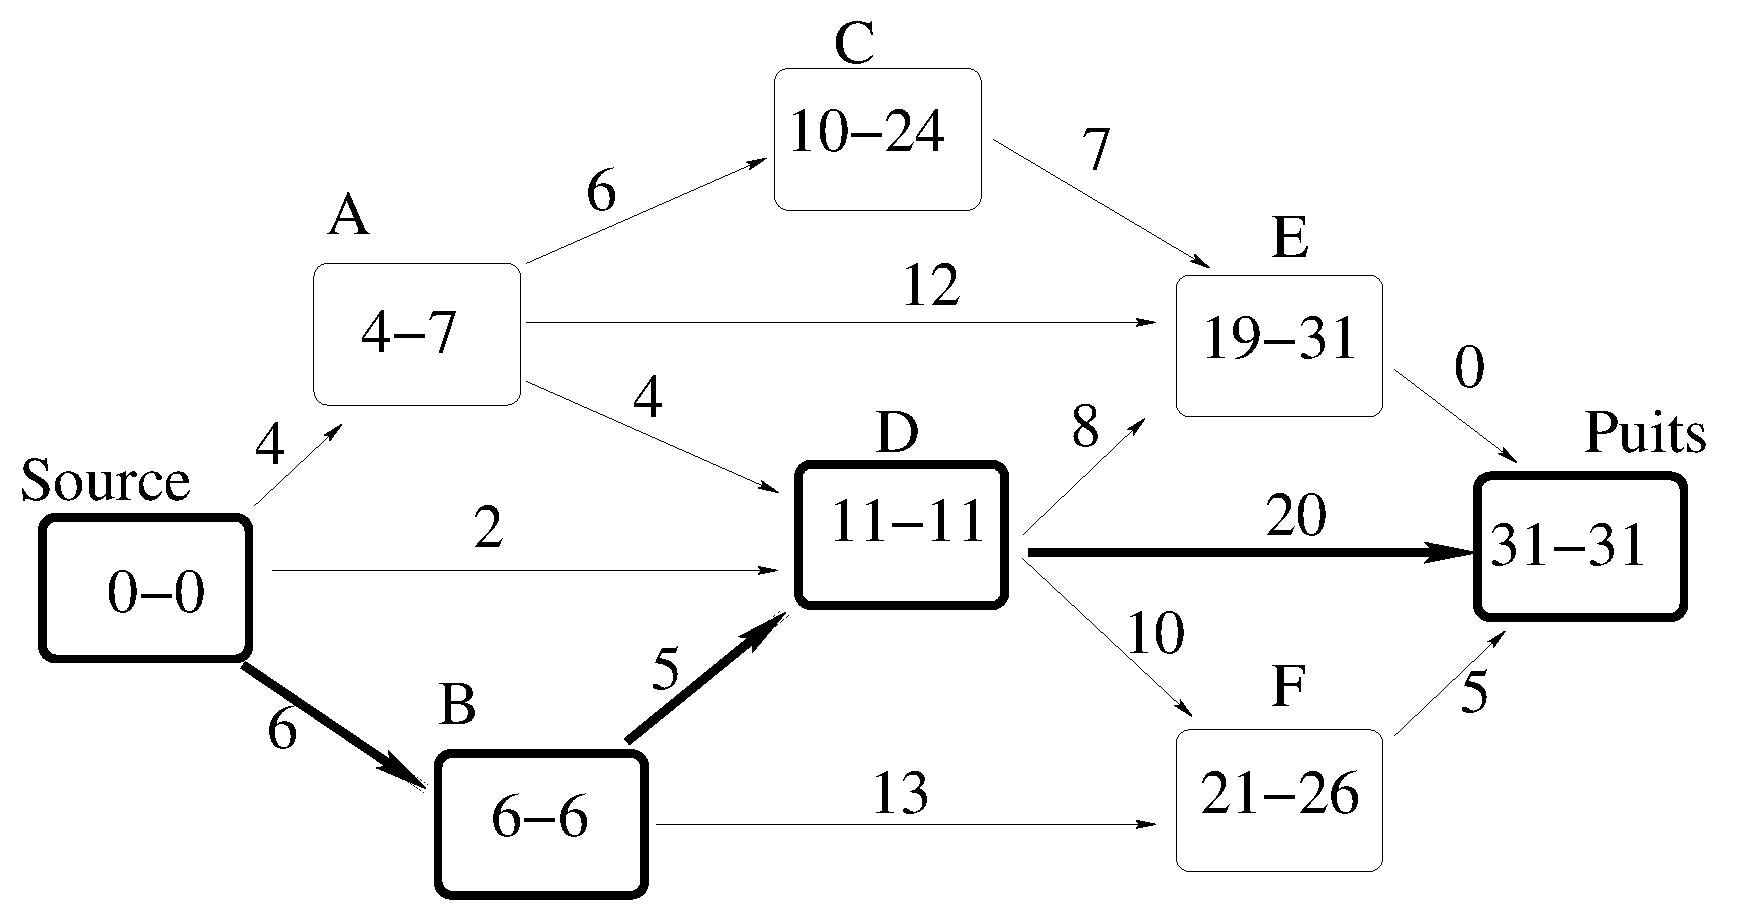
\includegraphics[width=0.75\linewidth]{critique2_solution.eps}
\end{center}

\begin{center}
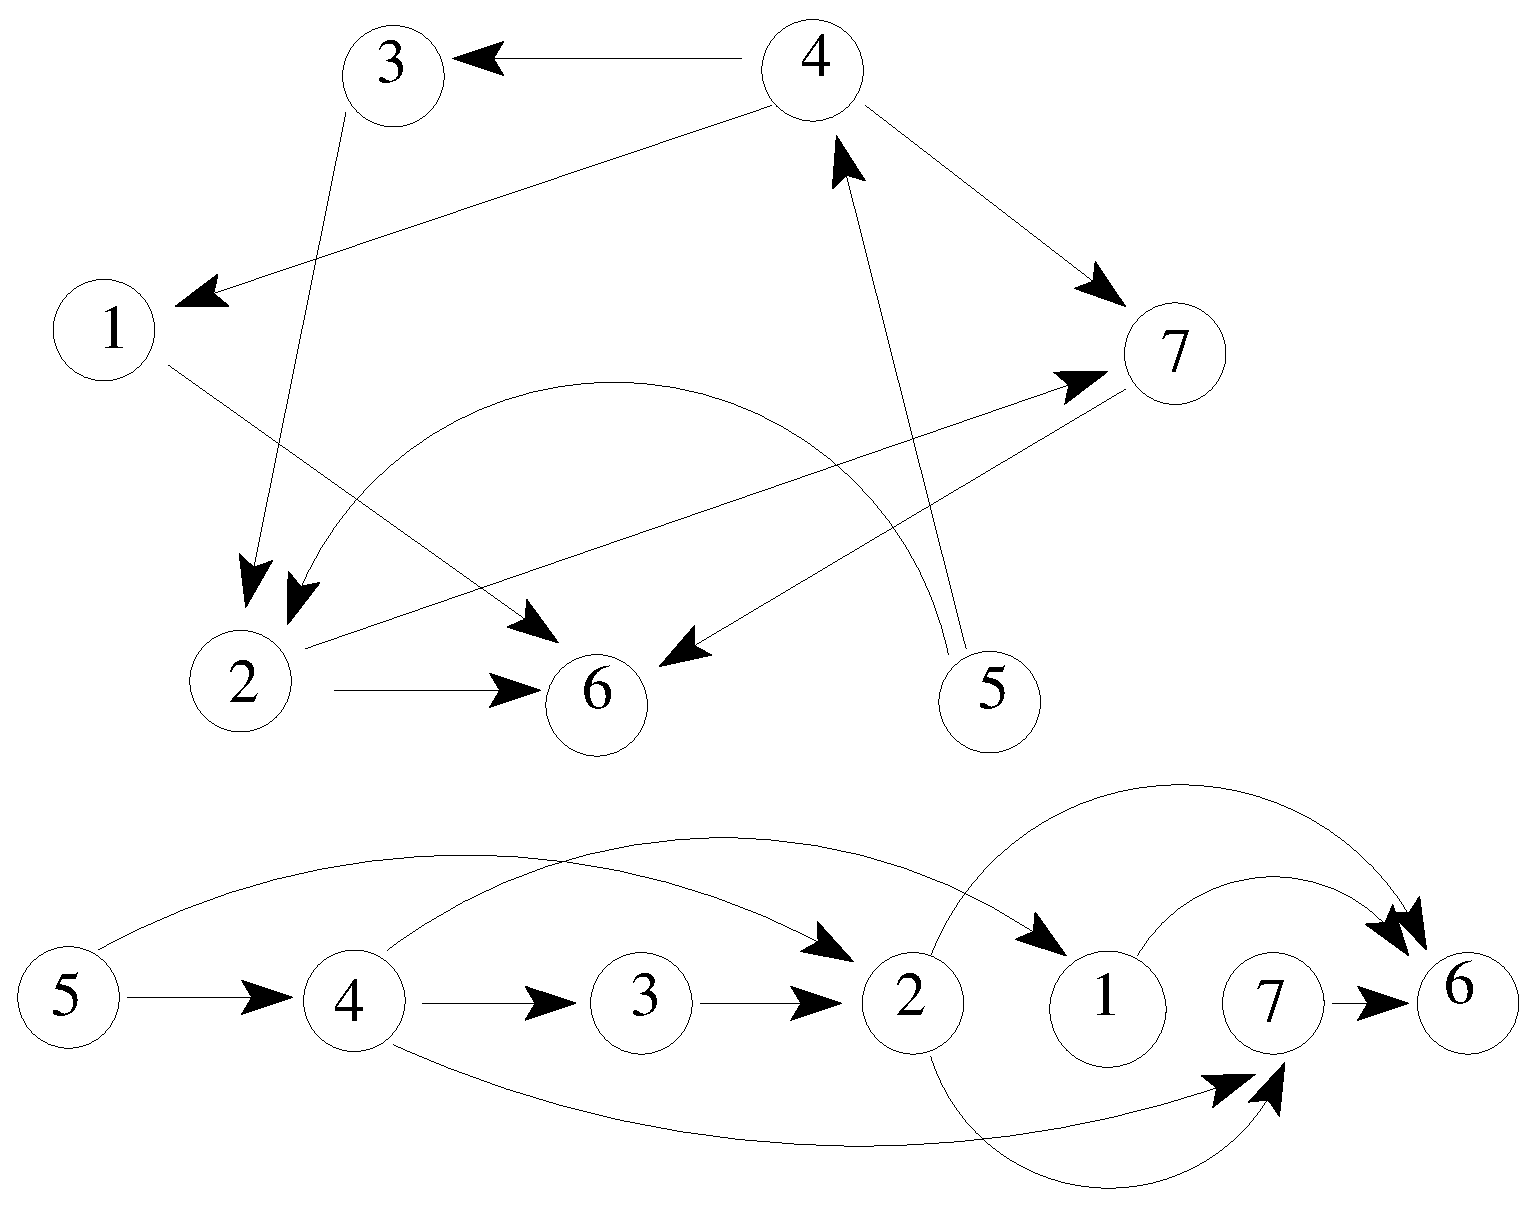
\includegraphics[width=0.6\linewidth]{tritopologique_corrige.eps}
\end{center}

\begin{center}
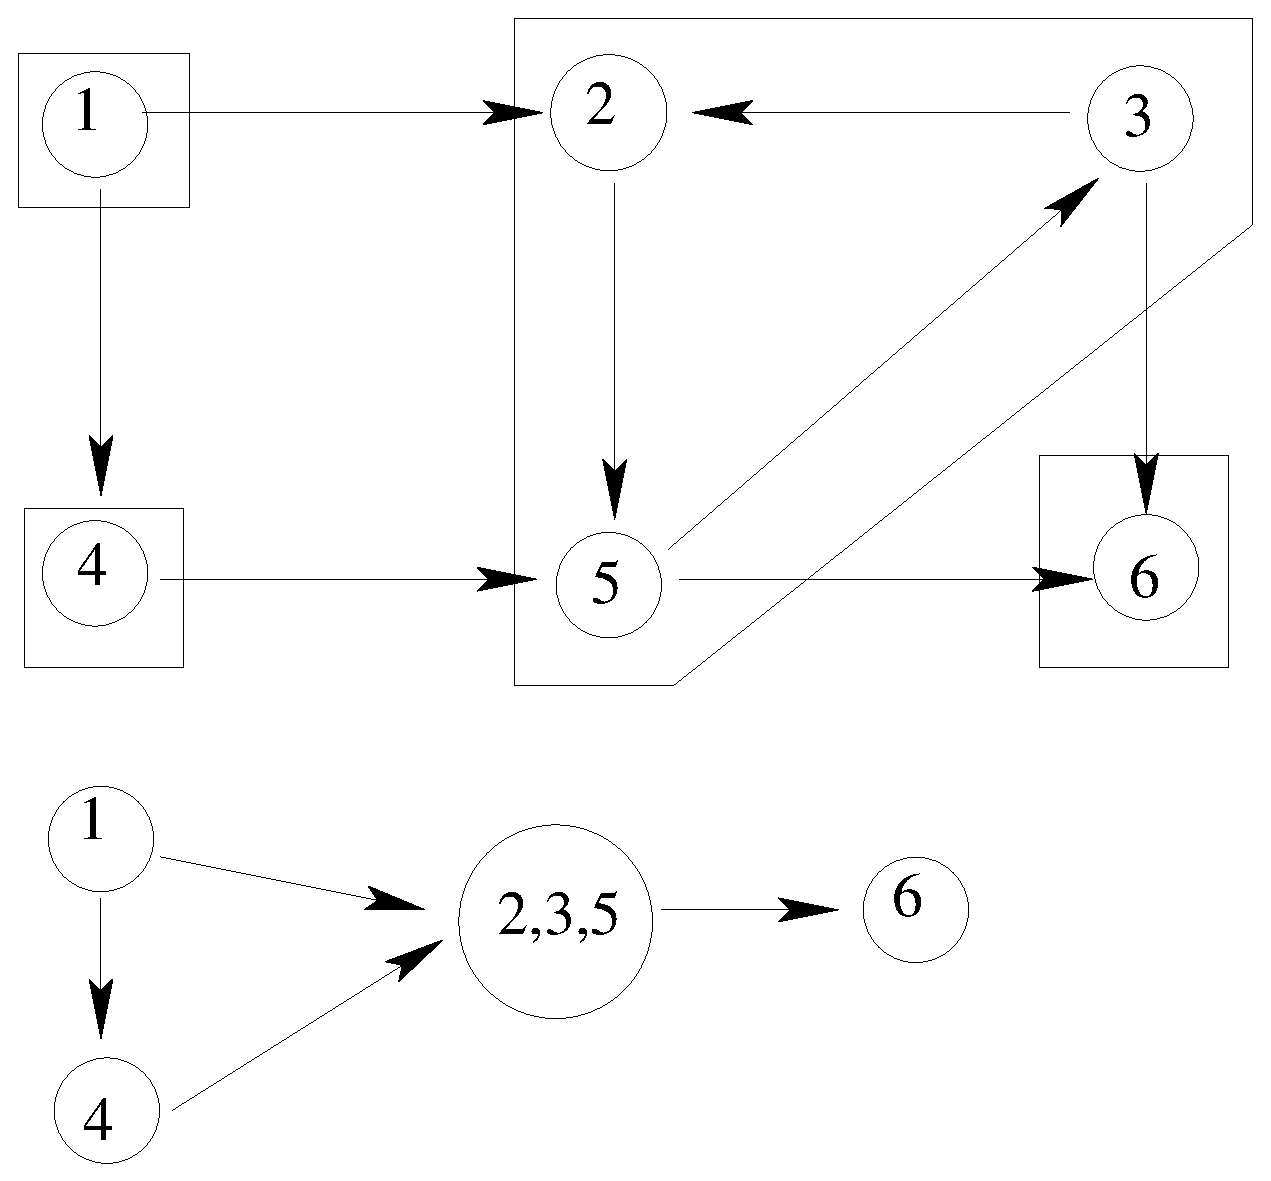
\includegraphics[width=0.5\linewidth]{cfc_bis.eps}
\end{center}
\newpage
{
\section{La toile}
Le graphe ci-dessous représente le web à la préhistoire.
Chaque sommet est une page, chaque arc est un lien. 
Les arcs $i\rightarrow j$ donnent la probabilité pour un internaute
de passer de la page $i$ à la page $j$ à l'instant suivant.
Soit $P=(p_i)$ le nombre d'internautes présents sur le sommet $i$ au temps $t$.
\begin{center}
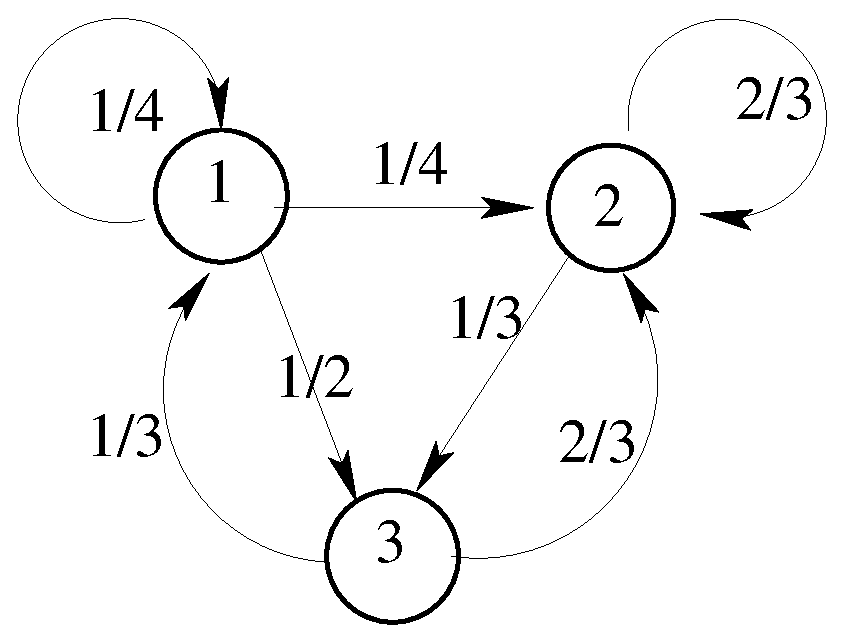
\includegraphics[width=0.5\linewidth]{markov.eps}
\end{center}

Exprimez par une relation matricielle $P'=(p_i')$,  le  nombre d'internautes présents sur les sommets $i$  au temps $t+1$.

Comment calculeriez-vous une distribution stationnaire~?
}
\end{document}
